\documentclass[12pt,a4paper]{article}

% --- packages ---
\usepackage{amsmath,amssymb,mathtools}
\usepackage{geometry}
\usepackage{microtype}
\usepackage{enumitem}
\usepackage{lmodern}
\usepackage[T1]{fontenc}
\usepackage{graphicx}
\usepackage{subcaption}
\graphicspath{{figures/}}
\usepackage{tikz}
\usetikzlibrary{arrows.meta}


\DeclareMathOperator{\sgn}{sgn}

% --- layout: generous white space like your sample ---
\geometry{margin=1in}
\setlength{\parskip}{0.9em}
\setlength{\parindent}{0pt}
\linespread{1.12}
\setlist[itemize]{topsep=0.3em,itemsep=0.2em}
\setlist[enumerate]{topsep=0.3em,itemsep=0.2em}

\DeclareMathOperator{\csch}{csch}
\DeclareMathOperator{\Arg}{Arg}
\DeclareMathOperator{\Res}{Res}
\DeclareMathOperator{\Log}{Log}

\newcommand{\C}{\mathbb{C}}
\newcommand{\R}{\mathbb{R}}

\newcommand{\axes}[3]{% center, x label, y label
	\draw[->,thin] (#1) -- ++(2.0,0) node[right] {#2};
	\draw[->,thin] (#1) -- ++(0,2.0) node[above] {#3};
}


% --- simple section styling helpers ---
\newcommand{\secdiv}{\par\vspace{0.6em}\hrule\par\vspace{0.8em}}
\newcommand{\subhead}[1]{\par\textbf{#1}\par\vspace{0.35em}}

\newcommand{\qed}{\hfill$\square$}

\title{\Large Entire Functions — Identity Theorem Applications \& a Polynomiality Criterion\\[0.3em]
	\large (spaced layout, matching the “Branches of $\log f$” style)}
\author{}
\date{}

\begin{document}
	\maketitle

\section*{A keyhole/Beta evaluation of \(\displaystyle \int_{0}^{\infty}\frac{x^{1/2}\log x}{(1+x)^2}\,dx\)}

\paragraph{Problem.}
Evaluate
\[
I=\int_{0}^{\infty}\frac{x^{1/2}\,\log x}{(1+x)^2}\,dx .
\]

\bigskip

\paragraph{Background.}
For \(0<a<2\) the Beta–Gamma identity gives
\[
F(a):=\int_{0}^{\infty}\frac{x^{a-1}}{(1+x)^2}\,dx
=B(a,2-a)=\Gamma(a)\Gamma(2-a).
\]
Differentiation under the parameter is legitimate here, and since
\(\dfrac{d}{da}x^{a-1}=x^{a-1}\log x\), we obtain integrals with a \(\log x\) factor
by differentiating \(F\).
We also use the digamma function \(\psi=\Gamma'/\Gamma\) and the values
\(\psi(\tfrac12)=-\gamma-2\log2\), \(\psi(\tfrac32)=\psi(\tfrac12)+2\).

\bigskip

\paragraph{Solution.}
Differentiate \(F\):
\[
F'(a)=\int_{0}^{\infty}\frac{x^{a-1}\log x}{(1+x)^2}\,dx
=\frac{d}{da}\big(\Gamma(a)\Gamma(2-a)\big)
=\Gamma(a)\Gamma(2-a)\big(\psi(a)-\psi(2-a)\big).
\]
We need \(I=F'(3/2)\).  Compute
\[
F\!\left(\tfrac32\right)
=\Gamma\!\left(\tfrac32\right)\Gamma\!\left(\tfrac12\right)
=\frac{\sqrt\pi}{2}\cdot\sqrt\pi=\frac{\pi}{2},
\qquad
\psi\!\left(\tfrac32\right)-\psi\!\left(\tfrac12\right)=2.
\]
Therefore
\[
I=F'\!\left(\tfrac32\right)
=\frac{\pi}{2}\cdot 2
=\boxed{\pi}.
\]

\bigskip

\paragraph{Remarks / extensions.}
\begin{itemize}
	\item Using the reflection form \(F(a)=(1-a)\pi/\sin(\pi a)\), one can also get
	\(F'(3/2)=\pi\) immediately since \(\cot(3\pi/2)=0\).
	\item In general,
	\[
	\int_{0}^{\infty}\frac{x^{a-1}\log x}{(1+x)^2}\,dx
	=\Gamma(a)\Gamma(2-a)\big(\psi(a)-\psi(2-a)\big),\qquad 0<a<2,
	\]
	and higher powers \((\log x)^m\) arise from higher \(a\)-derivatives.
\end{itemize}

\section*{Structure of the integrand \(\displaystyle F(z)=\frac{z^{1/2}\log z}{(1+z)^2}\) on the keyhole branch}

\paragraph{Branch choice (keyhole).}
Let \(\Log z=\ln|z|+i\,\Arg z\) with \(\Arg z\in(0,2\pi)\), so the branch cut is
the positive real axis \([0,\infty)\).
Set \(z^{1/2}=e^{\frac12\Log z}\) and \(\log z=\Log z\).
All maps below are considered on the slit plane
\[
\Omega:=\C\setminus[0,\infty).
\]

\bigskip

\paragraph{1.\ Numerator \(N(z)=z^{1/2}\log z\).}
\emph{Singular/branch points.}
\(z=0\) and \(z=\infty\) are branch points (from \(\sqrt z\) and \(\log z\)).

\emph{Zeros.}
\(\sqrt z=0\) only at \(z=0\) (excluded); \(\log z=0\) only at \(z=1\) (on the cut, excluded).
Hence \(N\) has no zeros in \(\Omega\).

\emph{Boundary values on the cut} (\(x>0\)):
\[
N_-(x)=\sqrt{x}\,\ln x,\qquad
N_+(x)=-\sqrt{x}\,(\ln x+i\,2\pi),
\]
so
\[
N_+(x)-N_-(x)=-\,2\sqrt{x}\,\ln x\;+\;i\,2\pi\sqrt{x}.
\]

\emph{Polar description.}
For \(z=re^{i\theta}\) with \(\theta\in(0,2\pi)\),
\[
N(z)=r^{1/2}e^{i\theta/2}\,\big(\ln r+i\theta\big).
\]
Rays (\(\theta=\) const) map to outward, gently bending trajectories.
Circles (\(r=\) const) map to spiral-like sweeps.

\bigskip

\paragraph{2.\ Denominator \(Q(z)=(1+z)^2\).}
\emph{Zeros/poles.}
Double zero at \(z=-1\); hence \(1/Q\) has a double pole at \(z=-1\) and is holomorphic elsewhere.
Near \(-1\),
\(\,(1+z)^{-2}=(z+1)^{-2}\) with magnitude \(\sim|z+1|^{-2}\) and argument \(-2\arg(z+1)\).

\bigskip

\paragraph{3.\ Full function \(F(z)=\dfrac{z^{1/2}\log z}{(1+z)^2}\).}
\emph{Domain.}
\(F\) is meromorphic on \(\Omega\) with a single isolated singularity at \(-1\).

\emph{Pole at \(-1\).}
Using \(\log(-1)=i\pi\), \((-1)^{1/2}=i\), we get \(N(-1)=i\cdot i\pi=-\pi\neq0\);
hence \(F\) has a \textbf{double pole} at \(z=-1\).

\emph{Zeros.}
Since \(N\) has no zeros in \(\Omega\), \(F\) has no zeros in \(\Omega\).

\emph{Branch points.}
\(0\) and \(\infty\) remain branch points (from the numerator).

\emph{Boundary values on \([0,\infty)\):}
\[
F_-(x)=\frac{\sqrt{x}\,\ln x}{(1+x)^2},\qquad
F_+(x)=\frac{-\sqrt{x}\,(\ln x+i\,2\pi)}{(1+x)^2},
\]
so the jump is
\[
F_+(x)-F_-(x)=\frac{-\,2\sqrt{x}\,\ln x+i\,2\pi\sqrt{x}}{(1+x)^2}.
\]
The imaginary part \( \dfrac{2\pi\sqrt{x}}{(1+x)^2}\) is exactly what integrates to \(\pi\) in the keyhole contour.

\emph{Asymptotics.}
Near \(z=0\): \(F(z)\sim z^{1/2}\log z\) (mild singularity).
As \(z\to\infty\): \(F(z)\sim z^{-3/2}\log z\) (decays; outer arc gives no contribution).
Near \(-1\): double pole determined by \(N(-1)=-\pi\).

\bigskip

\paragraph{Invertibility.}
Away from the branch set and \(-1\), \(F\) is locally conformal (typically \(F'\neq0\)),
but globally it is not single–valued across the cut and cannot be globally invertible on \(\C\).

\section*{Geometric mapping for \(F(z)=\dfrac{z^{1/2}\log z}{(1+z)^2}\) on the keyhole branch}

\paragraph{Branch and domain.}
Let \(\Log z=\ln|z|+i\,\Arg z\) with \(\Arg z\in(0,2\pi)\), so the branch cut is \([0,\infty)\).
Set \(z^{1/2}=e^{\frac12\Log z}\) and \(\log z=\Log z\).
All maps are considered on the slit plane
\[
\Omega=\C\setminus[0,\infty).
\]

\bigskip
\paragraph{1.\ Numerator \(N(z)=z^{1/2}\log z\).}
For \(z=re^{i\theta}\) with \(\theta\in(0,2\pi)\),
\[
N(z)=r^{1/2}e^{i\theta/2}\big(\ln r+i\theta\big).
\]
Zeros: none in \(\Omega\). Branch points: \(0,\infty\).

\emph{Boundary values on the cut} (\(x>0\)):
\[
N_-(x)=\sqrt{x}\,\ln x,\qquad
N_+(x)=-\sqrt{x}\,(\ln x+i\,2\pi),
\]
hence the jump
\[
N_+(x)-N_-(x)=-\,2\sqrt{x}\,\ln x+i\,2\pi\sqrt{x}.
\]

\emph{Images of simple sets.}
\begin{itemize}
\item Rays \(\theta=\theta_0\): \(w(r)=r^{1/2}e^{i\theta_0/2}(\ln r+i\theta_0)\) (outward, gently bending).
\item Circles \(r=r_0\): \(w(\theta)=r_0^{1/2}e^{i\theta/2}(\ln r_0+i\theta)\) (spiral-like).
\item Verticals \(x=x_0\): \(w(y)=(x_0^2+y^2)^{1/4}e^{i\theta(y)/2}\big(\tfrac12\ln(x_0^2+y^2)+i\theta(y)\big)\).
\item Horizontals \(y=y_0\): similar with \(x\) as parameter.
\end{itemize}

\bigskip
\paragraph{2.\ Denominator maps.}
\emph{(a) Squaring after translation: } \(Q(z)=(1+z)^2\).
Let \(\zeta=z+1\). Then \(w=\zeta^2\):
rays \(\arg\zeta=\phi\) go to rays of angle \(2\phi\);
circles \(|\zeta|=R\) go to circles \(|w|=R^2\);
lines through \(-1\) go to rays through the origin.

\emph{(b) Reciprocal used in \(F\): } \(H(z)=1/(1+z)^2=1/\zeta^2\).
There is a double pole at \(z=-1\).
Circles \(|z+1|=R\) map to circles \(|w|=1/R^2\).
Rays from \(-1\) map to rays with angle \(-2\arg(z+1)\).
Lines not through \(-1\) map to circles through the origin.

\bigskip
\paragraph{3.\ Full function \(F(z)=N(z)\,H(z)\).}
Domain \(\Omega\).
Double pole at \(-1\) (since \(N(-1)=i\cdot i\pi=-\pi\neq0\)).
Branch points at \(0,\infty\).
No zeros in \(\Omega\).

\emph{Boundary values on \([0,\infty)\):}
\[
F_-(x)=\frac{\sqrt{x}\,\ln x}{(1+x)^2},\qquad
F_+(x)=\frac{-\sqrt{x}\,(\ln x+i\,2\pi)}{(1+x)^2},
\]
so
\[
F_+(x)-F_-(x)=\frac{-\,2\sqrt{x}\,\ln x+i\,2\pi\sqrt{x}}{(1+x)^2}.
\]

\emph{Asymptotics.}
Near \(-1\): \(F(z)\sim -\pi/(z+1)^2\).
Near \(0\): \(F(z)\sim z^{1/2}\log z\).
At \(\infty\): \(F(z)\sim z^{-3/2}\log z\).

\emph{Images (qualitative).}
\begin{itemize}
\item Rays from \(-1\) remain rays (angle doubled and reversed by \(H\)), with magnitude dominated by \(1/|z+1|^2\).
\item Circles \(|z+1|=R\) map to circles \(|w|=|N(-1)|/R^2\) for small \(R\).
\item Verticals/horizontals map to smooth curves threading between the circles/rays produced by \(H\), reweighted pointwise by \(N(z)\).
\end{itemize}

\emph{Local inverse.}
Away from the branch set and the pole at \(-1\), \(F\) is locally conformal, but globally multivalued across the cut; no global inverse.

\section*{Plus/minus boundary values and jumps on the keyhole cut}


% --- Conventions and jump formulas for the keyhole branch ---

\subsection*{Conventions}

We work with the principal keyhole branch with cut along $[0,\infty)$:
\[
\Arg z\in(0,2\pi),\qquad \Log z=\ln|z|+i\,\Arg z,\qquad
z^{1/2}=e^{\frac12\Log z}.
\]

\begin{itemize}
\item For a point $x>0$ on the cut, define the one–sided boundary values
\[
f_{\pm}(x):=\lim_{\varepsilon\downarrow0} f\bigl(xe^{\pm i\varepsilon}\bigr),
\quad\text{with}\quad
f_{-}\ \text{(from below, }\Arg\to0^+),\ \ 
f_{+}\ \text{(from above, }\Arg\to2\pi^-).
\]

\item On this branch,
\[
\log(xe^{i0})=\ln x,\qquad
\log(xe^{i2\pi})=\ln x+i\,2\pi,
\]
and
\[
(xe^{i0})^{1/2}=+\sqrt{x},\qquad
(xe^{i2\pi})^{1/2}=e^{i\pi}\sqrt{x}=-\sqrt{x}.
\]
\end{itemize}

\bigskip

% ---------- BOX 1: Numerator ----------
\[
\boxed{%
\begin{aligned}
\textbf{Numerator } N(z)&=z^{1/2}\log z, \quad x>0: \\
N_-(x)&=\sqrt{x}\,\ln x,\\
N_+(x)&=-\sqrt{x}\,(\ln x+i\,2\pi),\\[2pt]
\Delta N(x)&:=N_+(x)-N_-(x)=-\,2\sqrt{x}\,\ln x\;+\;i\,2\pi\sqrt{x},\\
\frac{N_+(x)+N_-(x)}{2}&=-\,\sqrt{x}\,\ln x\;-\;i\,\pi\sqrt{x}.
\end{aligned}}
\]

\bigskip

% ---------- BOX 2: Full integrand ----------
\[
\boxed{%
\begin{aligned}
\textbf{Integrand } F(z)&=\frac{z^{1/2}\log z}{(1+z)^2}, \quad x>0: \\
F_-(x)&=\frac{\sqrt{x}\,\ln x}{(1+x)^2},\\
F_+(x)&=\frac{-\sqrt{x}\,(\ln x+i\,2\pi)}{(1+x)^2},\\[2pt]
\Delta F(x)&:=F_+(x)-F_-(x)=\frac{-\,2\sqrt{x}\,\ln x\;+\;i\,2\pi\sqrt{x}}{(1+x)^2},\\
\Im\Delta F(x)&=\frac{2\pi\sqrt{x}}{(1+x)^2}\quad\text{(keyhole contribution).}
\end{aligned}}
\]


\paragraph{Convention.}
We work with the principal keyhole branch with cut along $[0,\infty)$:
$\Arg z\in(0,2\pi)$.
For $x>0$ set
\[
f_\pm(x):=\lim_{\varepsilon\downarrow0} f\bigl(xe^{\pm i\varepsilon}\bigr),
\quad
f_-\ (\Arg\to 0^+),\;\; f_+\ (\Arg\to 2\pi^-).
\]
Then
\[
\log(xe^{i0})=\ln x,\qquad \log(xe^{i2\pi})=\ln x+i\,2\pi,
\]
\[
(xe^{i0})^{1/2}=+\sqrt{x},\qquad (xe^{i2\pi})^{1/2}=e^{i\pi}\sqrt{x}=-\sqrt{x}.
\]

\bigskip

\paragraph{Numerator \(N(z)=z^{1/2}\log z\).}
For $x>0$,
\[
N_-(x)=\sqrt{x}\,\ln x,\qquad
N_+(x)=-\sqrt{x}\,(\ln x+i\,2\pi).
\]
Hence the jump and average are
\[
\Delta N(x):=N_+(x)-N_-(x)=-\,2\sqrt{x}\,\ln x+i\,2\pi\sqrt{x},
\]
\[
\frac{N_+(x)+N_-(x)}{2}=-\,\sqrt{x}\,\ln x-i\,\pi\sqrt{x}.
\]
Equivalently,
\[
\Re\Delta N(x)=-2\sqrt{x}\,\ln x,\qquad
\Im\Delta N(x)=2\pi\sqrt{x}.
\]

\bigskip

\paragraph{Denominator \((1+z)^2\).}
This factor is single-valued across the cut:
\[
\bigl((1+x)^2\bigr)_+=(1+x)^2=\bigl((1+x)^2\bigr)_-.
\]

\bigskip

\paragraph{Full integrand \(F(z)=\dfrac{z^{1/2}\log z}{(1+z)^2}\).}
For $x>0$,
\[
F_-(x)=\frac{\sqrt{x}\,\ln x}{(1+x)^2},\qquad
F_+(x)=\frac{-\sqrt{x}\,(\ln x+i\,2\pi)}{(1+x)^2}.
\]
Therefore
\[
\Delta F(x):=F_+(x)-F_-(x)
=\frac{-\,2\sqrt{x}\,\ln x+i\,2\pi\sqrt{x}}{(1+x)^2},
\qquad
\frac{F_+(x)+F_-(x)}{2}
=\frac{-\,\sqrt{x}\,\ln x-i\,\pi\sqrt{x}}{(1+x)^2}.
\]
In particular,
\[
\Re\Delta F(x)=\frac{-2\sqrt{x}\,\ln x}{(1+x)^2},\qquad
\Im\Delta F(x)=\frac{2\pi\sqrt{x}}{(1+x)^2}.
\]

\medskip
\noindent
\emph{Remark.} In the keyhole contour evaluation of
$\displaystyle \int_0^\infty \frac{x^{1/2}\log x}{(1+x)^2}\,dx$,
it is precisely $\Im\Delta F(x)$ whose integral over $(0,\infty)$ produces the value $\pi$.


\section*{Beta--Gamma toolbox in the keyhole context}

\paragraph{Gamma function.}
For $\Re s>0$,
\[
\Gamma(s)=\int_{0}^{\infty} t^{\,s-1} e^{-t}\,dt.
\]
We shall use
\[
\Gamma(s+1)=s\,\Gamma(s),\qquad
\Gamma\Bigl(\frac12\Bigr)=\sqrt{\pi},\qquad
\Gamma\Bigl(\frac32\Bigr)=\frac12\sqrt{\pi},
\]
and, when convenient, Euler’s reflection formula
\[
\Gamma(s)\,\Gamma(1-s)=\frac{\pi}{\sin(\pi s)}.
\]

\bigskip

\paragraph{Beta function.}
For $\Re x,\Re y>0$,
\[
B(x,y)=\int_{0}^{1} t^{\,x-1}(1-t)^{\,y-1}\,dt,
\qquad
B(x,y)=\frac{\Gamma(x)\Gamma(y)}{\Gamma(x+y)}.
\]

\bigskip

\paragraph{Beta prime (the form that appears with a keyhole).}
Let $p>0$ and $0<a<p$. With $t=\dfrac{x}{1+x}$,
\[
\int_{0}^{\infty} \frac{x^{\,a-1}}{(1+x)^{p}}\,dx
=\int_{0}^{1} t^{\,a-1}(1-t)^{\,p-a-1}\,dt
=B(a,p-a)=\frac{\Gamma(a)\Gamma(p-a)}{\Gamma(p)}.
\]
In particular, for $p=2$ and $0<a<2$,
\[
F(a):=\int_{0}^{\infty}\frac{x^{\,a-1}}{(1+x)^2}\,dx
=\Gamma(a)\Gamma(2-a).
\]

\bigskip

\paragraph{Log factors via differentiation in the parameter.}
Since $\dfrac{d}{da}x^{a-1}=x^{a-1}\log x$, differentiation under the integral sign yields
\[
\int_{0}^{\infty}\frac{x^{\,a-1}\log x}{(1+x)^2}\,dx
=\frac{d}{da}\bigl[\Gamma(a)\Gamma(2-a)\bigr]
=\Gamma(a)\Gamma(2-a)\bigl(\psi(a)-\psi(2-a)\bigr),
\]
where $\psi=\Gamma'/\Gamma$ is the digamma function.
At $a=\tfrac32$,
\[
\Gamma\!\Bigl(\frac32\Bigr)\Gamma\!\Bigl(\frac12\Bigr)=\frac{\pi}{2},
\qquad
\psi\!\Bigl(\frac32\Bigr)-\psi\!\Bigl(\frac12\Bigr)=2,
\]
so
\[
\int_{0}^{\infty}\frac{x^{1/2}\log x}{(1+x)^2}\,dx
=\Bigl.\frac{d}{da}\,F(a)\Bigr|_{a=3/2}
=\frac{\pi}{2}\cdot 2
=\pi.
\]

\bigskip

% ---------- BOX A: Beta prime identity ----------
\[
\boxed{%
\int_{0}^{\infty}\frac{x^{\,a-1}}{(1+x)^{p}}\,dx
=B(a,p-a)=\frac{\Gamma(a)\Gamma(p-a)}{\Gamma(p)},
\quad
0<a<p.}
\]

\bigskip

% ---------- BOX B: Our case and its derivative ----------
\[
\boxed{%
F(a)=\int_{0}^{\infty}\frac{x^{\,a-1}}{(1+x)^2}\,dx
=\Gamma(a)\Gamma(2-a),\quad
F'(a)=\Gamma(a)\Gamma(2-a)\,\bigl(\psi(a)-\psi(2-a)\bigr).}
\]

\medskip
\noindent
\emph{Keyhole link.} The same $F(a)$ follows from a keyhole contour for
$\displaystyle \int_{\gamma}\frac{z^{\,a-1}}{(1+z)^2}\,dz$,
since the jump across the cut is $(1-e^{2\pi i a})$ times the positive–axis integral;
equating with $2\pi i$ times the residue at $z=-1$ produces $F(a)=\Gamma(a)\Gamma(2-a)$.
Differentiating in $a$ then yields the $\log x$ integral.


\section*{Geometry of the Gamma integrand \(I_s(z)=z^{\,s-1}e^{-z}\)}

\paragraph{Branch and domain in \(z\).}
Use the principal branch \(\Log z=\ln|z|+i\,\Arg z\) with \(\Arg z\in(-\pi,\pi)\), so the cut is \((-\infty,0]\).
Define \(z^{s-1}=e^{(s-1)\Log z}\).
Then \(I_s(z)\) is holomorphic on \(\Omega:=\C\setminus(-\infty,0]\), with branch points at \(0\) and \(\infty\).

\bigskip

\paragraph{Polar form and magnitude/phase (fixed \(s=\sigma+i\tau\)).}
For \(z=re^{i\theta}\) with \(\theta\in(-\pi,\pi)\),
\[
I_s(z)=r^{\sigma-1}e^{-r\cos\theta}\,
e^{\,i\{\tau\ln r+(\sigma-1)\theta-r\sin\theta\}}.
\]
Hence \(|I_s(z)|=r^{\sigma-1}e^{-r\cos\theta}\), which decays for \(\cos\theta>0\) and grows for \(\cos\theta<0\).

\bigskip

\paragraph{Images of characteristic sets in the \(z\)-plane (fixed \(s\)).}
\begin{itemize}
\item \textbf{Rays} \(\theta=\theta_0\): exponential damping if \(\cos\theta_0>0\), growth if \(\cos\theta_0<0\); phase twists like \(\tau\ln r\).
\item \textbf{Circles} \(r=r_0\): \(w(\theta)=r_0^{\sigma-1}e^{-r_0\cos\theta}\,e^{i((\sigma-1)\theta-r_0\sin\theta)}\), a wavy closed curve.
\item \textbf{Verticals/horizontals}: obtained by analytic variation of \(r,\theta\); bands map to the regions between the boundary images.
\end{itemize}

\bigskip

\paragraph{As a function of \(s\) (fixed \(z\in\Omega\)).}
\[
I_s(z)=e^{-z}\,e^{(s-1)\Log z}
=e^{-z}\,|z|^{\sigma-1}e^{i(\sigma-1)\Arg z}\,e^{i\tau\Arg z},
\]
so \(I_s(\cdot)\) is entire in \(s\).

\begin{itemize}
\item \textbf{Vertical lines} \(\sigma=\sigma_0\): \(|w|=e^{-\Re z}|z|^{\sigma_0-1}\) is constant, \(\arg w=(\sigma_0-1)\Arg z+\tau\,\Arg z-\Im z\).
If \(\Arg z\neq0\), \(\tau\)-variation traces a circle centred at the origin; if \(\Arg z=0\), the point is fixed.
\item \textbf{Horizontal lines} \(\tau=\tau_0\): \(|w|=e^{-\Re z}|z|^{\sigma-1}\) varies exponentially in \(\sigma\) and \(\arg w\) rotates linearly in \(\sigma\); thus a logarithmic spiral (degenerating to a ray when \(\Arg z=0\)).
\item \textbf{Bands}: vertical bands \(\sigma\in[a,b]\) map to annuli; horizontal bands \(\tau\in[c,d]\) map to spiral sectors.
\end{itemize}

\bigskip

\paragraph{From integrand to \(\Gamma(s)\).}
For \(\sigma>0\), \(\Gamma(s)=\int_0^{\infty} z^{\,s-1}e^{-z}\,dz\) converges absolutely.
By analytic continuation, \(\Gamma(s)\) becomes meromorphic in \(s\) with simple poles at \(s=0,-1,-2,\dots\), inherited from the \(z\to0^+\) behaviour of \(z^{s-1}\).

\bigskip

% ---- Boxed summaries ----

\[
\boxed{%
\begin{aligned}
\textbf{Fixed }s=\sigma+i\tau:\qquad
I_s(re^{i\theta})
&=r^{\sigma-1}e^{-r\cos\theta}\,e^{\,i\{\tau\ln r+(\sigma-1)\theta-r\sin\theta\}},\\[2pt]
|I_s|&=r^{\sigma-1}e^{-r\cos\theta}\ \ \text{(decay for }\cos\theta>0).
\end{aligned}}
\]

\bigskip

\[
\boxed{%
\begin{aligned}
\textbf{Fixed }z\in\Omega:\qquad
I_s(z)
&=e^{-z}\,|z|^{\sigma-1}\,e^{\,i\big((\sigma-1)\Arg z+\tau\Arg z - \Im z\big)},\\[2pt]
\sigma=\text{const}:&\ \text{circle (if }\Arg z\neq0),\quad
\tau=\text{const}: \text{log-spiral (ray if }\Arg z=0).
\end{aligned}}
\]



\paragraph{Quick geometry (what the pictures show).}
For fixed \(s=\sigma+i\tau\) and \(z=re^{i\theta}\),
\[
I_s(z)=r^{\sigma-1}e^{-r\cos\theta}\,e^{\,i\{\tau\ln r+(\sigma-1)\theta-r\sin\theta\}}.
\]
\begin{itemize}
\item \emph{Rays} \(\theta=\theta_0\) map to curves damped when \(\cos\theta_0>0\) and growing when \(\cos\theta_0<0\).
\item \emph{Circles} \(|z|=R\) map to wavy closed loops modulated by \(e^{-R\cos\theta}\).
\item For fixed \(z\in\mathbb{C}\setminus(-\infty,0]\): \(|I_s(z)|=e^{-\Re z}|z|^{\sigma-1}\).
Thus vertical \(s\)-lines \(\sigma=\sigma_0\) sweep a \emph{circle} (if \(\Arg z\neq0\)) and
horizontal \(s\)-lines \(\tau=\tau_0\) sweep a \emph{logarithmic spiral} (degenerates to a ray if \(\Arg z=0\)).
\end{itemize}

\vspace{0.6em}
\begin{figure}[h]
\centering
\begin{subfigure}[t]{0.48\textwidth}
\centering

\includegraphics[width=\linewidth]{figures/Downloads_.figs_gamma_integrand_zmap_rays.png}
\caption{Images of several rays in the \(z\)-plane (fixed \(s\)).}
\end{subfigure}\hfill
\begin{subfigure}[t]{0.48\textwidth}
\centering

\includegraphics[width=\linewidth]{figures/Downloads_.figs_gamma_integrand_zmap_circles.png}
\caption{Images of circles \(|z|=R\) (fixed \(s\)).}
\end{subfigure}
\caption{Mapping \(z\mapsto I_s(z)=z^{\,s-1}e^{-z}\); branch cut along \((-\infty,0]\).}
\label{fig:zmap}
\end{figure}

\vspace{0.8em}
\begin{figure}[h]
\centering
\begin{subfigure}[t]{0.48\textwidth}
\centering

\includegraphics[width=\linewidth]{figures/Downloads_.figs_gamma_integrand_smap_vertical.png}
\caption{\(s\)-map for \(\sigma=\sigma_0\) (vary \(\tau\)): circle at fixed \(|I_s(z)|\).}
\end{subfigure}\hfill
\begin{subfigure}[t]{0.48\textwidth}
\centering

\includegraphics[width=\linewidth]{figures/Downloads_.figs_gamma_integrand_smap_horizontal.png}
\caption{\(s\)-map for \(\tau=\tau_0\) (vary \(\sigma\)): logarithmic spiral.}
\end{subfigure}
\caption{Mapping \(s\mapsto I_s(z)\) for a fixed \(z\) with \(\Arg z\neq0\).}
\label{fig:smap}
\end{figure}

\vspace{0.8em}
\begin{figure}[h]
\centering

\includegraphics[width=0.78\linewidth]{figures/Downloads_.figs_gamma_integrand_z_heatmap.png}
\caption{Compressed magnitude \(\log_{10}\!\bigl(1+|I_s(z)|\bigr)\) in the \(z\)-plane (fixed \(s\)); branch cut masked.}
\label{fig:heat}
\end{figure}

\section*{Factor analysis of the Gamma integrand \(I_s(z)=z^{\,s-1}e^{-z}\)}

\paragraph{Branch and domain.}
Use \(\Log z=\ln|z|+i\,\Arg z\) with \(\Arg z\in(-\pi,\pi)\); the slit is \((-\infty,0]\).
Set \(A(z)=z^{\,s-1}=e^{(s-1)\Log z}\) and \(E(z)=e^{-z}\).
Then \(I_s=A\cdot E\) is holomorphic on \(\Omega=\C\setminus(-\infty,0]\).

\subsection*{A) Algebraic factor \(A(z)=z^{\,s-1}\), \(s=\sigma+i\tau\)}
For \(z=re^{i\theta}\) (\(\theta\in(-\pi,\pi)\)),
\[
A(z)=r^{\sigma-1}\,e^{-\tau\theta}\,e^{\,i(\tau\ln r+(\sigma-1)\theta)},\qquad
|A(z)|=r^{\sigma-1}e^{-\tau\theta}.
\]
Branch points at \(0\) and \(\infty\); no poles.

\emph{Cut values.} For \(x>0\),
\[
A_\pm(-x)=x^{\,s-1}e^{(s-1)(\pm i\pi)}=x^{\sigma-1}\,e^{\mp\pi\tau}\,e^{\pm i\pi(\sigma-1)},
\quad
\frac{A_+(-x)}{A_-(-x)}=e^{-2\pi\tau}e^{i2\pi(\sigma-1)}.
\]

\emph{Images.} Rays \(\theta=\theta_0\) map to logarithmic spirals (radius \(r^{\sigma-1}e^{-\tau\theta_0}\), angle \(\tau\ln r\)).
Circles \(|z|=R\) map to loops with amplitude \(R^{\sigma-1}e^{-\tau\theta}\).

\subsection*{B) Exponential factor \(E(z)=e^{-z}\)}
Entire; \(|E(z)|=e^{-\Re z}\), \(\arg E(z)=-\,\Im z\).
Vertical lines \(\Re z=c\) map to circles of radius \(e^{-c}\); horizontal lines \(\Im z=y_0\) map to rays of fixed angle \(-y_0\) with radial scale \(e^{-x}\).

\subsection*{C) Product \(I_s(z)=A(z)E(z)\)}
\[
I_s(re^{i\theta})=r^{\sigma-1}e^{-r\cos\theta}\;
e^{\,i\{\tau\ln r+(\sigma-1)\theta-r\sin\theta\}},
\qquad
|I_s|=r^{\sigma-1}e^{-r\cos\theta}.
\]
Thus there is exponential decay in the right half-plane (\(\cos\theta>0\)) and exponential growth in the left half-plane (\(\cos\theta<0\)).

\emph{Cut values.} Since \(E(-x)=e^{x}\),
\[
I_{s,\pm}(-x)=x^{\sigma-1}\,e^{x}\,e^{\mp\pi\tau}\,e^{\pm i\pi(\sigma-1)},\qquad
\frac{I_{s,+}(-x)}{I_{s,-}(-x)}=e^{-2\pi\tau}e^{i2\pi(\sigma-1)}.
\]

\emph{Set images.} 
Rays \(\theta=\theta_0\) are damped or amplified according to \(e^{-r\cos\theta_0}\), with algebraic twist \(\tau\ln r\).
Circles \(|z|=R\) produce undulating loops with envelope \(e^{-R\cos\theta}\).
Vertical/horizontal lines inherit the circle/ray structure of \(E\) modulated by the spiralling of \(A\).

\section*{Differentiating the parameter integral and the Beta--Gamma link}

\paragraph{Step 1: Parameter integral.}
For \(a\in(0,2)\),
\[
F(a):=\int_{0}^{\infty}\frac{x^{a-1}}{(1+x)^2}\,dx.
\]
Since \(\dfrac{d}{da}x^{a-1}=x^{a-1}\log x\) and the integrand is dominated near \(0\) and \(\infty\),
\[
F'(a)=\int_{0}^{\infty}\frac{x^{a-1}\log x}{(1+x)^2}\,dx.
\]
In particular,
\[
\int_{0}^{\infty}\frac{x^{1/2}\log x}{(1+x)^2}\,dx
=F'\!\left(\frac{3}{2}\right).
\]

\paragraph{Step 2: Evaluate \(F(a)\) via Beta.}
With \(t=\dfrac{x}{1+x}\),
\[
F(a)=\int_{0}^{\infty}\frac{x^{a-1}}{(1+x)^2}\,dx
=\int_{0}^{1} t^{a-1}(1-t)^{2-a-1}\,dt
=B(a,2-a).
\]
Euler’s identity gives \(B(x,y)=\dfrac{\Gamma(x)\Gamma(y)}{\Gamma(x+y)}\), hence
\[
F(a)=\Gamma(a)\,\Gamma(2-a).
\]

\paragraph{Step 3: Differentiate \(F(a)\).}
Let \(\psi=\Gamma'/\Gamma\) denote the digamma function. Then
\[
F'(a)=\frac{d}{da}\bigl[\Gamma(a)\Gamma(2-a)\bigr]
=\Gamma(a)\Gamma(2-a)\bigl(\psi(a)-\psi(2-a)\bigr).
\]
At \(a=\tfrac32\),
\[
\Gamma\!\Bigl(\tfrac32\Bigr)=\frac12\sqrt{\pi},\quad
\Gamma\!\Bigl(\tfrac12\Bigr)=\sqrt{\pi},\quad
\psi\!\Bigl(\tfrac32\Bigr)-\psi\!\Bigl(\tfrac12\Bigr)=2,
\]
so
\[
F'\!\Bigl(\tfrac32\Bigr)
=\Gamma\!\Bigl(\tfrac32\Bigr)\Gamma\!\Bigl(\tfrac12\Bigr)\cdot 2
=\frac{\sqrt{\pi}}{2}\cdot \sqrt{\pi}\cdot 2
=\pi.
\]
Therefore,
\[
\boxed{\ \int_{0}^{\infty}\frac{x^{1/2}\log x}{(1+x)^2}\,dx=\pi\ }.
\]

\paragraph{Step 4: Keyhole derivation.}
Consider \(\displaystyle \oint_\gamma \frac{z^{a-1}}{(1+z)^2}\,dz\) on the keyhole contour with the principal branch.
The jump across the cut is \((1-e^{2\pi i a})\) times the real integral; the only pole inside is at \(z=-1\).
Equating the contour integral to \(2\pi i\) times the residue yields \(F(a)=\Gamma(a)\Gamma(2-a)\).
Differentiating in \(a\) gives the integral with \(\log x\).


\section*{The Beta function: theory and tools}

\paragraph{Definition (Euler).}
For $\Re x>0$ and $\Re y>0$,
\[
B(x,y):=\int_{0}^{1} t^{\,x-1}(1-t)^{\,y-1}\,dt,
\qquad B(x,y)=B(y,x).
\]

\paragraph{Relation to the Gamma function (Euler’s identity).}
For $\Re x,\Re y>0$,
\[
B(x,y)=\frac{\Gamma(x)\,\Gamma(y)}{\Gamma(x+y)}.
\]
\emph{Proof sketch.} Using
$\Gamma(x)\Gamma(y)=\iint_{(0,\infty)^2} u^{x-1}v^{y-1}e^{-(u+v)}\,du\,dv$,
substitute $u=rs$, $v=r(1-s)$ with $r\in(0,\infty)$, $s\in(0,1)$.
The Jacobian is $r$, and the integral factorizes as
$\bigl[\int_{0}^{\infty} r^{x+y-1}e^{-r}dr\bigr]\cdot\bigl[\int_{0}^{1} s^{x-1}(1-s)^{y-1}ds\bigr]$,
i.e.\ $\Gamma(x+y)\,B(x,y)$.

\paragraph{Analytic continuation.}
Via $B(x,y)=\Gamma(x)\Gamma(y)/\Gamma(x+y)$, the Beta function is meromorphic on $\C^2$
with simple poles where $\Gamma(x)$ or $\Gamma(y)$ does (at nonpositive integers), modulo cancellations when $x+y$ is also a nonpositive integer.

\paragraph{Beta prime (improper) integral.}
For $p>0$ and $0<\Re a<\Re p$,
\[
\int_{0}^{\infty}\frac{x^{\,a-1}}{(1+x)^{p}}\,dx
=\int_{0}^{1} t^{\,a-1}(1-t)^{\,p-a-1}\,dt
=B(a,p-a)=\frac{\Gamma(a)\Gamma(p-a)}{\Gamma(p)}.
\]
This follows from $t=\frac{x}{1+x}$.

\paragraph{Recurrences and special values.}
From $\Gamma(x+1)=x\,\Gamma(x)$,
\[
B(x+1,y)=\frac{x}{x+y}\,B(x,y),\qquad
B(x,y+1)=\frac{y}{x+y}\,B(x,y).
\]
If $m,n\in\mathbb{N}$,
\[
B(m,n)=\frac{(m-1)!(n-1)!}{(m+n-1)!}.
\]

\paragraph{Trigonometric form (Wallis integrals).}
For $\Re \alpha,\Re \beta>0$,
\[
\int_{0}^{\pi/2}\sin^{\alpha-1}\theta\,\cos^{\beta-1}\theta\,d\theta
=\frac{1}{2}\,B\!\left(\frac{\alpha}{2},\frac{\beta}{2}\right).
\]

\paragraph{Differentiation formulas (digamma).}
With $\psi=\Gamma'/\Gamma$,
\[
\partial_x\log B(x,y)=\psi(x)-\psi(x+y),\qquad
\partial_y\log B(x,y)=\psi(y)-\psi(x+y),
\]
hence
\[
\partial_x B(x,y)=B(x,y)\bigl[\psi(x)-\psi(x+y)\bigr],\qquad
\partial_y B(x,y)=B(x,y)\bigl[\psi(y)-\psi(x+y)\bigr].
\]
These generate integrals with $\log t$ or $\log(1-t)$; via $t=\frac{x}{1+x}$ they yield
$\log x$ integrals on $(0,\infty)$.

\paragraph{Probability viewpoint (normalizations).}
On $[0,1]$, the $\mathrm{Beta}(x,y)$ density is $t^{x-1}(1-t)^{y-1}/B(x,y)$.
On $(0,\infty)$, the Beta prime density is proportional to $x^{a-1}(1+x)^{-p}$, normalized by $B(a,p-a)$.

\paragraph{Asymptotics.}
Using Stirling’s expansion for $\Gamma$,
\[
\log B(x,y)=\log\Gamma(x)+\log\Gamma(y)-\log\Gamma(x+y),
\]
which yields precise growth estimates for large parameters.

\section*{The Beta function: theory and tools}

\paragraph{Definition (Euler).}
For $\Re x>0$ and $\Re y>0$,
\[
B(x,y):=\int_{0}^{1} t^{\,x-1}(1-t)^{\,y-1}\,dt,
\qquad B(x,y)=B(y,x).
\]

\paragraph{Relation to the Gamma function (Euler’s identity).}
For $\Re x,\Re y>0$,
\[
B(x,y)=\frac{\Gamma(x)\,\Gamma(y)}{\Gamma(x+y)}.
\]
\emph{Proof sketch.} Using
$\Gamma(x)\Gamma(y)=\iint_{(0,\infty)^2} u^{x-1}v^{y-1}e^{-(u+v)}\,du\,dv$,
substitute $u=rs$, $v=r(1-s)$ with $r\in(0,\infty)$, $s\in(0,1)$.
The Jacobian is $r$, and the integral factorizes as
$\bigl[\int_{0}^{\infty} r^{x+y-1}e^{-r}dr\bigr]\cdot\bigl[\int_{0}^{1} s^{x-1}(1-s)^{y-1}ds\bigr]$,
i.e.\ $\Gamma(x+y)\,B(x,y)$.

\paragraph{Analytic continuation.}
Via $B(x,y)=\Gamma(x)\Gamma(y)/\Gamma(x+y)$, the Beta function is meromorphic on $\C^2$
with simple poles where $\Gamma(x)$ or $\Gamma(y)$ does (at nonpositive integers), modulo cancellations when $x+y$ is also a nonpositive integer.

\paragraph{Beta prime (improper) integral.}
For $p>0$ and $0<\Re a<\Re p$,
\[
\int_{0}^{\infty}\frac{x^{\,a-1}}{(1+x)^{p}}\,dx
=\int_{0}^{1} t^{\,a-1}(1-t)^{\,p-a-1}\,dt
=B(a,p-a)=\frac{\Gamma(a)\Gamma(p-a)}{\Gamma(p)}.
\]
This follows from $t=\frac{x}{1+x}$.

\paragraph{Recurrences and special values.}
From $\Gamma(x+1)=x\,\Gamma(x)$,
\[
B(x+1,y)=\frac{x}{x+y}\,B(x,y),\qquad
B(x,y+1)=\frac{y}{x+y}\,B(x,y).
\]
If $m,n\in\mathbb{N}$,
\[
B(m,n)=\frac{(m-1)!(n-1)!}{(m+n-1)!}.
\]

\paragraph{Trigonometric form (Wallis integrals).}
For $\Re \alpha,\Re \beta>0$,
\[
\int_{0}^{\pi/2}\sin^{\alpha-1}\theta\,\cos^{\beta-1}\theta\,d\theta
=\frac{1}{2}\,B\!\left(\frac{\alpha}{2},\frac{\beta}{2}\right).
\]

\paragraph{Differentiation formulas (digamma).}
With $\psi=\Gamma'/\Gamma$,
\[
\partial_x\log B(x,y)=\psi(x)-\psi(x+y),\qquad
\partial_y\log B(x,y)=\psi(y)-\psi(x+y),
\]
hence
\[
\partial_x B(x,y)=B(x,y)\bigl[\psi(x)-\psi(x+y)\bigr],\qquad
\partial_y B(x,y)=B(x,y)\bigl[\psi(y)-\psi(x+y)\bigr].
\]
These generate integrals with $\log t$ or $\log(1-t)$; via $t=\frac{x}{1+x}$ they yield
$\log x$ integrals on $(0,\infty)$.

\paragraph{Probability viewpoint (normalizations).}
On $[0,1]$, the $\mathrm{Beta}(x,y)$ density is $t^{x-1}(1-t)^{y-1}/B(x,y)$.
On $(0,\infty)$, the Beta prime density is proportional to $x^{a-1}(1+x)^{-p}$, normalized by $B(a,p-a)$.

\paragraph{Asymptotics.}
Using Stirling’s expansion for $\Gamma$,
\[
\log B(x,y)=\log\Gamma(x)+\log\Gamma(y)-\log\Gamma(x+y),
\]
which yields precise growth estimates for large parameters.

\section*{Problem}
By considering
\[
\int_{\Gamma_n} \frac{\pi\,dw}{w^{2}\sin(\pi w)},
\]
where $\Gamma_n$ is the square with vertices $\pm(n+\tfrac12)(1\pm i)$ in~$\C$, show that
\[
\frac{\pi^2}{12}
\;=\;
1-\frac14+\frac19-\frac1{16}+\cdots
\;=\;
\sum_{k=1}^{\infty}\frac{(-1)^{k+1}}{k^{2}}.
\]
(Assume there is $C>0$ such that $|\csc(\pi w)|\le C$ on $\Gamma_n$, uniformly in $n$.)

\section*{Background}
\begin{itemize}
	\item \textbf{Residue theorem:} $\displaystyle \int_{\partial D} f(z)\,dz=2\pi i\sum \operatorname{Res}(f;\text{poles in }D)$.
	\item \textbf{Zeros of $\sin(\pi w)$:} simple zeros at each $k\in\mathbb Z$; $\sin(\pi w)=\pi(-1)^k(w-k)+O((w-k)^2)$.
	\item \textbf{Series for $\csc$:} as $z\to0$,
	\[
	\csc z=\frac1{z}+\frac{z}{6}+\frac{7z^{3}}{360}+\cdots,
	\qquad
	\Rightarrow\qquad
	\pi\,\csc(\pi w)=\frac1{w}+\frac{\pi^{2}w}{6}+O(w^{3}).
	\]
	\item \textbf{Decay on $\Gamma_n$:} with $|\csc(\pi w)|\le C$ and $|w|\asymp n$ on $\Gamma_n$,
	\[
	\left|\frac{\pi}{w^{2}\sin(\pi w)}\right|
	=\left|\frac{\pi\,\csc(\pi w)}{w^{2}}\right|
	\le \frac{\pi C}{|w|^{2}}
	\lesssim \frac{1}{n^{2}},
	\]
	while $\operatorname{length}(\Gamma_n)=O(n)$, so $\int_{\Gamma_n}\to0$ as $n\to\infty$.
\end{itemize}

\section*{Solution}
Let $f(w)=\dfrac{\pi}{w^{2}\sin(\pi w)}$. The poles inside $\Gamma_n$ are all integers $k$ with $|k|\le n$, together with $w=0$ (higher order because of $w^{2}$). By the estimate above,
\[
\lim_{n\to\infty}\int_{\Gamma_n} f(w)\,dw=0.
\]
Hence, by the residue theorem,
\[
0=\lim_{n\to\infty}\int_{\Gamma_n} f(w)\,dw
=2\pi i\left(\operatorname{Res}(f;0)+\sum_{k\in\mathbb Z\setminus\{0\}}\operatorname{Res}(f;k)\right).
\]

\paragraph{Residues at $k\neq0$.}
Since $\sin(\pi w)\sim \pi(-1)^k(w-k)$,
\[
\operatorname{Res}(f;k)
=\lim_{w\to k}(w-k)\frac{\pi}{w^{2}\sin(\pi w)}
=\frac{\pi}{k^{2}}\cdot\frac{1}{\pi(-1)^k}
=\frac{(-1)^k}{k^{2}}.
\]

\paragraph{Residue at $0$.}
Using $\pi\,\csc(\pi w)=\dfrac1{w}+\dfrac{\pi^{2}w}{6}+O(w^{3})$,
\[
f(w)=\frac{\pi\,\csc(\pi w)}{w^{2}}
=\frac{1}{w^{3}}+\frac{\pi^{2}}{6}\,\frac{1}{w}+O(w),
\]
so $\operatorname{Res}(f;0)=\dfrac{\pi^{2}}{6}$.

\paragraph{Summing residues.}
Thus
\[
0=\operatorname{Res}(f;0)+\sum_{k\in\mathbb Z\setminus\{0\}}\frac{(-1)^k}{k^{2}}
=\frac{\pi^{2}}{6}+2\sum_{k=1}^{\infty}\frac{(-1)^k}{k^{2}}.
\]
Therefore

\[
\sum_{k=1}^\infty \frac{(-1)^{k+1}}{k^2}=\frac{\pi^2}{12} \hfill\square
\]


\section*{Geometry of the denominator \(D(w)=w^{2}\sin(\pi w)\)}

\subsection*{Domain, zeros, and image}

\textbf{Entirety.} \(D:\C\to\C\) is entire, being a product of the polynomial \(w^{2}\) and the entire function \(\sin(\pi w)\).

\medskip
\textbf{Zeros.} Zeros occur at the zeros of \(w^{2}\) and of \(\sin(\pi w)\):
\[
\sin(\pi w)=0 \iff w\in\mathbb{Z}.
\]
Hence
\[
\boxed{\ \operatorname{ord}_{0}D=3\quad\text{and}\quad \operatorname{ord}_{k}D=1\ \text{for all}\ k\in\mathbb{Z}\setminus\{0\}\ }.
\]
(At \(w=0\) you get a double zero from \(w^{2}\) and a simple zero from \(\sin(\pi w)\).)

\medskip
\textbf{Image and preimages.} By Picard’s theorem and basic properties of sine, \(D\) attains every complex value (indeed also \(0\)) with an infinite discrete preimage (counted with multiplicity). Thus
\[
\boxed{\ \mathrm{Im}(D)=\C,\quad D^{-1}(a)\ \text{is infinite and discrete for every}\ a\in\C\ }.
\]

\subsection*{Decomposition of \(\sin(\pi w)\) and the ellipse--hyperbola grid}

Write \(w=x+iy\) and
\[
\sin(\pi w)=\sin(\pi x)\cosh(\pi y)+i\,\cos(\pi x)\sinh(\pi y)=:u+iv.
\]

\paragraph{Images of vertical lines \(x=x_{0}\).}
For fixed \(x=x_{0}\) and varying \(y\in\mathbb{R}\),
\[
u=\sin(\pi x_{0})\cosh(\pi y),\qquad v=\cos(\pi x_{0})\sinh(\pi y).
\]
Eliminating \(y\) via \(\cosh^{2}-\sinh^{2}=1\) gives the confocal hyperbola
\[
\boxed{\ \frac{u^{2}}{\sin^{2}(\pi x_{0})}-\frac{v^{2}}{\cos^{2}(\pi x_{0})}=1\ }.
\]
Degeneracies: if \(x_{0}\in\mathbb{Z}\) then \(u\equiv0\) (the imaginary axis); if \(x_{0}\in\frac12+\mathbb{Z}\) then \(v\equiv0\) (the real axis).

\paragraph{Images of horizontal lines \(y=y_{0}\).}
For fixed \(y=y_{0}\) and varying \(x\in\mathbb{R}\),
\[
u=\sin(\pi x)\cosh(\pi y_{0}),\qquad v=\cos(\pi x)\sinh(\pi y_{0}),
\]
and the relation
\[
\boxed{\ \frac{u^{2}}{\cosh^{2}(\pi y_{0})}+\frac{v^{2}}{\sinh^{2}(\pi y_{0})}=1\ }
\]
describes a family of confocal ellipses.  

\emph{Conclusion:} \(\sin(\pi w)\) maps the rectangular grid in the \(w\)-plane to an orthogonal net of ellipses (from \(y=\text{const}\)) and hyperbolas (from \(x=\text{const}\)) in the \(q\)-plane, \(q=\sin(\pi w)\).

\subsection*{Effect of multiplying by \(w^{2}\): \(D(w)=w^{2}\sin(\pi w)\)}

For \(w=re^{i\phi}\),
\[
w^{2}=r^{2}e^{i\,2\phi}\quad\Rightarrow\quad \text{local scaling by }r^{2}\ \text{and rotation by }2\phi.
\]
Therefore the ellipse/hyperbola images produced by \(\sin(\pi w)\) are subsequently pointwise scaled by \(|w|^{2}\) and rotated by \(2\Arg w\). Globally they are no longer confocal families, but remain smooth curves. Near \(w=0\), the triple zero forces strong collapse of images.

\medskip
\textbf{On the real axis} \((y=0)\):
\[
D(x)=x^{2}\sin(\pi x)\in\mathbb{R},\qquad \text{zeros at }x\in\mathbb{Z},\ \text{peaks near }x=k+\tfrac12.
\]

\textbf{On the imaginary axis} \((w=iy)\):
\[
\sin(\pi i y)=i\sinh(\pi y),\qquad D(iy)=-(y^{2})\,i\,\sinh(\pi y),
\]
hence
\[
|D(iy)|=y^{2}\,|\sinh(\pi y)|\sim \frac12\,y^{2}e^{\pi|y|}\qquad(|y|\to\infty),
\]
i.e.\ extremely rapid growth in the vertical direction.

\subsection*{Critical points and extrema}

Differentiate:
\[
D'(w)=2w\sin(\pi w)+\pi w^{2}\cos(\pi w).
\]
Thus either \(w=0\) or
\[
\boxed{\ 2\sin(\pi w)+\pi w\cos(\pi w)=0\quad\Longleftrightarrow\quad \tan(\pi w)=-\frac{\pi w}{2}\ }.
\]
This transcendental equation has an infinite discrete set of solutions (roughly near half-integers on the real axis and their vertical translates); these are the saddle/extremal locations of \(D\).

\subsection*{Asymptotics and band structure}

As \(|y|\to\infty\),
\[
\sin(\pi w)=\tfrac12 e^{\pi|y|}\,e^{\,i\,(\pi x\,\sgn y)}\,(1+o(1)),
\]
hence
\[
D(w)=w^{2}\sin(\pi w)\sim \frac{|w|^{2}}{2}\,e^{\pi|y|}\,e^{\,i\,\big(\pi x\,\sgn y+2\Arg w\big)},
\qquad |y|\to\infty.
\]
Consequently
\[
\frac{1}{D(w)}=O\!\left(\frac{e^{-\pi|y|}}{|w|^{2}}\right),
\]
which is exactly the decay that makes the large–square contour integral of \(\pi/(w^{2}\sin\pi w)\) tend to \(0\).

\medskip
\textbf{Bands/strips.} Preimages of annular or strip-like sets in the \(q=\sin(\pi w)\) plane are bounded by the ellipse/hyperbola families above. Multiplication by \(w^{2}\) then stretches and rotates these images locally. There is no global preservation of “band” geometry, but the map remains conformal off the zeros, with local dilation \(|D'(w)|\).

\subsection*{One-line summary for quick reference}

\[
\boxed{
	\begin{array}{l}
		\text{Entire } D(w)=w^{2}\sin(\pi w);\ \text{zeros: }\operatorname{ord}_{0}=3,\ \operatorname{ord}_{k}=1\ (k\neq0).\\[0.3em]
		\sin(\pi w):\ \text{vertical lines }\to\text{ hyperbolas},\ \text{horizontal lines }\to\text{ ellipses}.\\[0.3em]
		\text{Factor }w^{2}:\ \text{local scale }|w|^{2}\ \text{and rotation }2\Arg w.\\[0.3em]
		|D(iy)|\sim \tfrac12 y^{2}e^{\pi|y|};\ \ D'(w)=0\ \Leftrightarrow\ \tan(\pi w)=-\pi w/2\ (\text{or }w=0).
	\end{array}
}
\]

% assumes \usepackage{amsmath,amssymb} in the preamble
\section*{Effect of multiplying by \(w^{2}\): local rotation and scale}

Let
\[
q(w)=\sin(\pi w)=u(w)+i\,v(w),\qquad D(w)=w^{2}\,q(w).
\]
Fix a horizontal line \(y=y_{0}\) in the \(w\)-plane and parametrize it by
\[
w(x)=x+i\,y_{0},\qquad x\in\mathbb{R}.
\]
Under \(q\), this line maps to a \emph{confocal ellipse} in the \(q\)-plane:
\[
u(x)=\sin(\pi x)\cosh(\pi y_{0}),\qquad
v(x)=\cos(\pi x)\sinh(\pi y_{0}),\qquad
\frac{u^{2}}{\cosh^{2}(\pi y_{0})}+\frac{v^{2}}{\sinh^{2}(\pi y_{0})}=1.
\]

\subsection*{Pointwise action of \(w^{2}\)}
Write
\[
w(x)^{2}=a(x)+i\,b(x),\qquad
a(x)=x^{2}-y_{0}^{2},\quad b(x)=2\,x\,y_{0}.
\]
Then the post–multiplication curve is
\[
D\bigl(w(x)\bigr)
=(a+ib)\,(u+iv)
=\bigl( a\,u - b\,v \bigr)
+ i\,\bigl( b\,u + a\,v \bigr).
\]
Equivalently, in real form,
\[
\begin{pmatrix}
	\Re D \\[2pt] \Im D
\end{pmatrix}
=
\underbrace{
	\begin{pmatrix}
		a(x) & -\,b(x)\\[2pt]
		b(x) & \ \ a(x)
\end{pmatrix}}_{\displaystyle =\ |w(x)|^{2}
	\begin{psmallmatrix}
		\cos(2\arg w(x)) & -\sin(2\arg w(x))\\
		\sin(2\arg w(x)) & \ \cos(2\arg w(x))
\end{psmallmatrix}}
\begin{pmatrix}
	u(x)\\[2pt] v(x)
\end{pmatrix}.
\]
Thus, at each parameter value \(x\),
\[
w(x)^{2}=|w(x)|^{2}\,e^{\,i\,2\arg w(x)}
\]
acts as a similarity transformation:
\[
\text{scale by }|w(x)|^{2}\quad\text{and}\quad
\text{rotate by }2\arg w(x).
\]

\paragraph{Key consequence.}
Because \(a(x),b(x)\) (equivalently \(|w(x)|,\arg w(x)\)) depend on the parameter \(x\), the ellipse is \emph{not} rigidly rotated into another ellipse. Instead, it is \emph{deformed}: each point is rotated by a \emph{different} angle \(2\arg w(x)\) and scaled by a \emph{different} factor \(|w(x)|^{2}\).
Only \emph{locally} (near some \(x=x_{0}\)) can one approximate
\[
w(x)^{2}\approx w(x_{0})^{2},
\]
in which case the ellipse segment is approximately a uniformly rotated-and-scaled copy (rotation \(\approx 2\arg w(x_{0})\), scale \(\approx |w(x_{0})|^{2}\)).

\subsection*{Special cases and intuition}
\begin{itemize}
	\item \textbf{Real axis} (\(y_{0}=0\)): \(w(x)^{2}=x^{2}>0\) is real and positive. There is no rotation; only a varying scale \(x^{2}\).
	\item \textbf{Far vertical lines} (\(|y_{0}|\gg 1\)): for large \(|x|\), \(\arg w(x)\) varies slowly and \(|w(x)|^{2}\sim x^{2}+y_{0}^{2}\) is large; the dominant effect is strong (but slowly varying) magnification.
	\item \textbf{Matrix viewpoint}: multiplying \(q=u+iv\) by \(w^{2}=a+ib\) equals the real linear map
	\[
	(u,v)\mapsto \bigl(au-bv,\ bu+av\bigr),
	\]
	i.e.\ a rotation by \(\arg(w^{2})=2\arg w\) followed by a scale \(|w^{2}|=|w|^{2}\), both depending on the base point.
\end{itemize}

\paragraph{Bottom line.}
Multiplication by \(w^{2}\) applies a \emph{pointwise} similarity (rotation \(2\arg w\), scale \(|w|^{2}\)). The ellipse coming from \(\sin(\pi w)\) is therefore not carried to a single rigidly rotated ellipse; it becomes a smoothly \emph{twisted} oval that is, \emph{locally}, a rotated-and-scaled copy of the original

\section*{Problem}
Evaluate the principal value
\[
\operatorname{PV}\int_{-\infty}^{\infty}\frac{(x+1)\cos x}{x^{2}+1}\,dx.
\]

\section*{Background}
\begin{itemize}
	\item \textbf{Even/odd symmetry.} $\cos x$ is even. The decomposition
	\[
	\frac{x+1}{x^{2}+1}=\frac{x}{x^{2}+1}+\frac{1}{x^{2}+1}
	\]
	shows that $\dfrac{x}{x^{2}+1}$ is odd and $\dfrac{1}{x^{2}+1}$ is even. Hence
	$\dfrac{x\cos x}{x^{2}+1}$ is odd, while $\dfrac{\cos x}{x^{2}+1}$ is even.
	\item \textbf{Standard transform.} For $a\in\mathbb R$,
	\[
	\int_{-\infty}^{\infty}\frac{\cos(ax)}{x^{2}+1}\,dx=\pi e^{-|a|}.
	\]
	A contour proof uses $f(z)=\dfrac{e^{iaz}}{z^{2}+1}$ on a large semicircle
	in the upper half-plane when $a>0$, with residue at $z=i$.
\end{itemize}

\section*{Solution}
Split the integrand:
\[
\frac{(x+1)\cos x}{x^{2}+1}
=\frac{x\cos x}{x^{2}+1}+\frac{\cos x}{x^{2}+1}.
\]
The first term is odd, so its principal value integral over $\mathbb R$ is $0$.
Therefore
\[
\operatorname{PV}\!\int_{-\infty}^{\infty}\frac{(x+1)\cos x}{x^{2}+1}\,dx
=\int_{-\infty}^{\infty}\frac{\cos x}{x^{2}+1}\,dx
=\pi e^{-1}
=\frac{\pi}{e}.
\]

\paragraph{(Residue check, optional).}
Consider $f(z)=\dfrac{e^{iz}}{z^{2}+1}$ and integrate over the upper semicircle.
The only enclosed pole is at $z=i$, with residue $\mathrm{Res}(f;i)=\dfrac{e^{i\cdot i}}{2i}
=\dfrac{e^{-1}}{2i}$. Jordan’s lemma gives
\[
\int_{-\infty}^{\infty}\frac{e^{ix}}{x^{2}+1}\,dx=2\pi i\cdot\frac{e^{-1}}{2i}=\pi e^{-1}.
\]
Taking real parts yields $\displaystyle \int_{-\infty}^{\infty}\frac{\cos x}{x^{2}+1}\,dx=\pi e^{-1}$.

\section*{Numerator, denominator, and the meromorphic map}

Let
\[
N(z)=(z+1)\cos z,\qquad D(z)=z^{2}+1,\qquad F(z)=\frac{N(z)}{D(z)}.
\]

\subsection*{Denominator \(D(z)=z^{2}+1\)}
\begin{itemize}
	\item Entire, surjective onto \(\C\). For any \(w\in\C\), \(D(z)=w \iff z=\pm\sqrt{\,w-1\,}\) (two preimages with multiplicity).
	\item Zeros (simple) at \(z=\pm i\). Hence \(F\) has simple poles at \(\pm i\).
	\item Geometry: \(z\mapsto z^{2}\) doubles angles on rays, sends circles \(|z|=R\) to \(|w|=R^{2}\), and lines not through \(0\) to parabolas; the \(+1\) translates images by \(1\).
\end{itemize}

\subsection*{Numerator \(N(z)=(z+1)\cos z\)}
\begin{itemize}
	\item Entire; image is all of \(\C\).
	\item Zeros: \(z=-1\) and \(z=\tfrac{\pi}{2}+k\pi\) for \(k\in\mathbb Z\); all simple.
	\item Write \(\cos(x+iy)=\cos x\cosh y - i\sin x\sinh y =: u+iv\).
	\begin{itemize}
		\item Horizontal lines \(y=y_{0}\): \(\displaystyle \frac{u^{2}}{\cosh^{2}(\pi y_{0})}+\frac{v^{2}}{\sinh^{2}(\pi y_{0})}=1\) (ellipses).
		\item Vertical lines \(x=x_{0}\): \(\displaystyle \frac{u^{2}}{\cos^{2}(\pi x_{0})}-\frac{v^{2}}{\sin^{2}(\pi x_{0})}=1\) (hyperbolas, degenerate to axes at integers/half-integers).
		\item Multiplication by \(z+1=|z+1|e^{i\arg(z+1)}\) applies a \emph{pointwise} similarity: scale \(|z+1|\), rotation \(\arg(z+1)\). It does not rigidly rotate an entire ellipse.
	\end{itemize}
\end{itemize}

\subsection*{The quotient \(F(z)=N(z)/D(z)\)}
\begin{itemize}
	\item Domain \(\C\setminus\{\pm i\}\); simple poles at \(\pm i\).
	\item Zeros: simple at \(z=-1\) and \(z=\tfrac{\pi}{2}+k\pi\), \(k\in\mathbb Z\).
	\item Growth: \(|F(z)|\sim e^{|\Im z|}/|z|\) for large \(|\Im z|\); along \(\R\), \(F(x)=O(1/|x|)\).
	\item Image/preimages: meromorphic map with infinite discrete fibers \(F^{-1}(w)\) for each \(w\in\widehat{\C}\) (except possibly a discrete exceptional set).
	\item Mapping of canonical sets: start from the ellipse/hyperbola net of \(\cos z\), then apply the pointwise similarity by \(z+1\), and finally the rational warp by \(1/(z^{2}+1)\); curves are bent and blown up near \(z=\pm i\) and cross the zero lattice.
\end{itemize}

\paragraph{Restriction to the real axis.}
\[
F(x)=\frac{(x+1)\cos x}{x^{2}+1}
=\underbrace{\frac{x\cos x}{x^{2}+1}}_{\text{odd}}
+\underbrace{\frac{\cos x}{x^{2}+1}}_{\text{even}}.
\]
The principal value of the odd part over \(\R\) is \(0\), while
\(\displaystyle \int_{-\infty}^{\infty}\frac{\cos x}{x^{2}+1}dx=\pi e^{-1}\).


\section*{Principal value computation}

We evaluate
\[
\operatorname{PV}\int_{-\infty}^{\infty}\frac{(x+1)\cos x}{x^{2}+1}\,dx
:=\lim_{R\to\infty}\int_{-R}^{R}\frac{(x+1)\cos x}{x^{2}+1}\,dx.
\]

\paragraph{Even/odd split.}
\[
\frac{(x+1)\cos x}{x^{2}+1}
=\underbrace{\frac{x\cos x}{x^{2}+1}}_{\text{odd}}
+\underbrace{\frac{\cos x}{x^{2}+1}}_{\text{even}}.
\]
Hence
\[
\int_{-R}^{R}\frac{x\cos x}{x^{2}+1}\,dx=0\quad(\forall R),\qquad
\operatorname{PV}\int_{-\infty}^{\infty}\frac{x\cos x}{x^{2}+1}\,dx=0,
\]
and (the even part being absolutely integrable)
\[
\operatorname{PV}\int_{-\infty}^{\infty}\frac{(x+1)\cos x}{x^{2}+1}\,dx
=\int_{-\infty}^{\infty}\frac{\cos x}{x^{2}+1}\,dx.
\]

\paragraph{Residue evaluation of the cosine integral.}
For $a>0$, define
\[
I(a)=\int_{-\infty}^{\infty}\frac{e^{iax}}{x^{2}+1}\,dx.
\]
Integrating over a large upper semicircle and using Jordan’s lemma, the arc integral tends to $0$, and the only pole inside is $z=i$ with
\[
\operatorname{Res}\!\left(\frac{e^{iaz}}{z^{2}+1};\,z=i\right)
=\frac{e^{iai}}{2i}=\frac{e^{-a}}{2i}.
\]
By the residue theorem, $I(a)=2\pi i\cdot \frac{e^{-a}}{2i}=\pi e^{-a}$ for $a>0$, so
\[
\int_{-\infty}^{\infty}\frac{\cos(ax)}{x^{2}+1}\,dx=\Re I(a)=\pi e^{-a}.
\]
With $a=1$,
\[
\int_{-\infty}^{\infty}\frac{\cos x}{x^{2}+1}\,dx=\pi e^{-1}.
\]

\paragraph{Conclusion.}
\[
\operatorname{PV}\int_{-\infty}^{\infty}\frac{(x+1)\cos x}{x^{2}+1}\,dx
=\frac{\pi}{e}.
\]

\paragraph{Odd vs.\ even parts.}
Decompose
\[
\frac{(x+1)\cos x}{x^{2}+1}
=\underbrace{\frac{x\cos x}{x^{2}+1}}_{\displaystyle f(x)}
+\underbrace{\frac{\cos x}{x^{2}+1}}_{\displaystyle g(x)}.
\]

\noindent
\textbf{(1) The odd part vanishes.}
Since \(\cos(-x)=\cos x\) and \((-x)/(x^{2}+1)=-x/(x^{2}+1)\), we have
\[
f(-x)=-\,f(x),
\]
so \(f\) is odd. Therefore, for every \(R>0\),
\[
\int_{-R}^{R}\frac{x\cos x}{x^{2}+1}\,dx=0,
\]
and hence
\[
\operatorname{PV}\int_{-\infty}^{\infty}\frac{x\cos x}{x^{2}+1}\,dx=0.
\]

\noindent
\textbf{(2) The even part does not vanish.}
Here
\[
g(-x)=g(x),
\]
so \(g\) is even and
\[
\int_{-R}^{R}\frac{\cos x}{x^{2}+1}\,dx
=2\int_{0}^{R}\frac{\cos x}{x^{2}+1}\,dx \neq 0 \ \text{in general}.
\]
Moreover \(g\) is absolutely integrable (since \(|g(x)|\le 1/(x^{2}+1)\in L^{1}(\mathbb R)\)), so its PV equals the ordinary improper integral, which can be evaluated e.g.\ by residues:
\[
\int_{-\infty}^{\infty}\frac{\cos x}{x^{2}+1}\,dx=\pi e^{-1}.
\]

\noindent
\textbf{Conclusion.}
\[
\operatorname{PV}\int_{-\infty}^{\infty}\frac{(x+1)\cos x}{x^{2}+1}\,dx
=\underbrace{0}_{\text{odd part}}
+\underbrace{\pi e^{-1}}_{\text{even part}}
=\frac{\pi}{e}.
\]

\section*{Contour for \(\displaystyle \int_{-\infty}^{\infty}\frac{e^{ix}}{x^{2}+1}\,dx\) and Jordan bound}

\subsection*{Contour picture}
\begin{figure}[h]
	\centering
	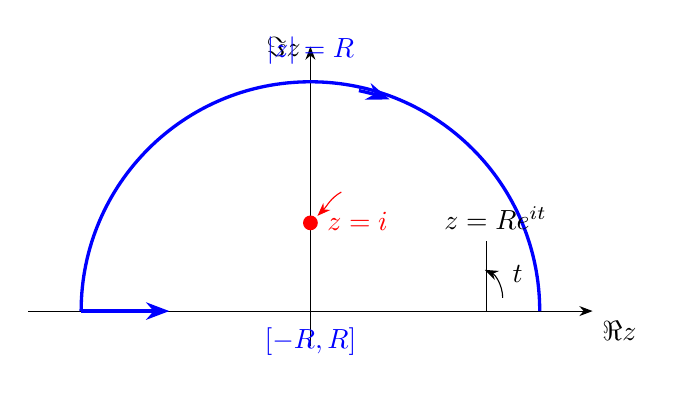
\begin{tikzpicture}[scale=1.12,>=Stealth]
		
		% axes
		\draw[->] (-3.2,0) -- (3.2,0) node[below right] {$\Re z$};
		\draw[->] (0,-0.4) -- (0,3.0) node[left] {$\Im z$};
		
		% big semicircle of radius R
		\def\R{2.6}
		\draw[very thick,blue] (-\R,0) arc (180:0:\R);     % arc
		\draw[very thick,blue,->] (-\R,0) -- (-1.6,0);     % orientation mark on real line
		\draw[very thick,blue,->] (0.55,2.50) arc (78:70:\R); % orientation mark on arc
		
		% labels
		\node[blue] at (0,2.95) {$|z|=R$};
		\node[blue] at (0,-0.35) {$[-R,R]$};
		
		% pole at z=i
		\filldraw[red] (0,1) circle (2.2pt);
		\node[red,right] at (0.08,1.02) {$z=i$};
		\draw[red,->] (0.35,1.35) to[out=210,in=45] (0.08,1.08);
		
		% parameter/angle on arc
		\draw (2.0,0) -- (2.0,0.8);
		\draw[->] (2.18,0.15) arc (0:65:0.35);
		\node at (2.35,0.42) {$t$};
		\node at (2.1,1.05) {$z=Re^{it}$};
		
	\end{tikzpicture}
	\caption{Upper semicircle contour for \(f(z)=\dfrac{e^{iz}}{z^{2}+1}\). The only enclosed pole is at \(z=i\).}
\end{figure}

\subsection*{Jordan–lemma bound on the arc}
Let \(C_R\) be the upper semicircle \(|z|=R\) with parameter \(z=Re^{it}\), \(t\in[0,\pi]\). We estimate the arc integral
\[
I_R^{\mathrm{arc}}=\int_{C_R}\frac{e^{iz}}{z^{2}+1}\,dz .
\]

\paragraph{Step 1: Parameterize.}
With \(z=Re^{it}\) we have \(dz=iRe^{it}\,dt\) and \(|dz|=R\,dt\).

\paragraph{Step 2: Exponential decay on the arc (Jordan).}
\[
\bigl|e^{iz}\bigr|=e^{-\Im z}=e^{-R\sin t},\qquad t\in[0,\pi].
\]

\paragraph{Step 3: Denominator bound for \(R>1\).}
\[
|z^{2}+1|=\bigl|R^{2}e^{i2t}+1\bigr|\ge R^{2}-1 .
\]

\paragraph{Step 4: Combine.}
\[
\left|I_R^{\mathrm{arc}}\right|
=\left|\int_{0}^{\pi}\frac{e^{iRe^{it}}}{R^{2}e^{i2t}+1}\,iRe^{it}\,dt\right|
\le \int_{0}^{\pi}\frac{e^{-R\sin t}}{R^{2}-1}\,R\,dt
=\frac{R}{R^{2}-1}\int_{0}^{\pi} e^{-R\sin t}\,dt .
\]

\paragraph{Step 5: Elementary estimate for \(\int_{0}^{\pi}e^{-R\sin t}\,dt\).}
Using \(\sin t\ge \tfrac{2t}{\pi}\) on \([0,\tfrac{\pi}{2}]\) and symmetry,
\[
\int_{0}^{\pi}e^{-R\sin t}\,dt
\le 2\int_{0}^{\pi/2} e^{-R\cdot(2t/\pi)}\,dt
=2\cdot\frac{\pi}{2R}\bigl(1-e^{-R}\bigr)
\le \frac{\pi}{R}.
\]

\paragraph{Step 6: Conclusion.}
\[
\boxed{\;
	\left|I_R^{\mathrm{arc}}\right|
	\le \frac{R}{R^{2}-1}\cdot\frac{\pi}{R}
	=\frac{\pi}{R^{2}-1}\xrightarrow[R\to\infty]{}0\; }.
\]

Therefore, the contour integral equals the real–axis integral, and by the residue theorem
\[
\int_{-\infty}^{\infty}\frac{e^{ix}}{x^{2}+1}\,dx
=2\pi i\,\mathrm{Res}\!\left(\frac{e^{iz}}{z^{2}+1};\,z=i\right)
=2\pi i\cdot\frac{e^{ii}}{2i}
=\pi e^{-1}.
\]
Taking real parts yields
\[
\int_{-\infty}^{\infty}\frac{\cos x}{x^{2}+1}\,dx=\pi e^{-1}.
\]
``

\section*{Sector contour proof of \(\displaystyle \int_{0}^{\infty}\frac{dx}{1+x^{n}}=\frac{\pi}{n}\csc\!\bigl(\frac{\pi}{n}\bigr)\) for \(n\ge2\)}

Let \(f(z)=\dfrac{1}{1+z^{n}}\) and let \(\Gamma_R\) be the contour consisting of
\([0,R]\), the circular arc \(|z|=R\) with \(\arg z\in[0,2\pi/n]\), and
\([Re^{2\pi i/n},0]\). The poles of \(f\) are the \(n\)th roots of \(-1\),
\[
z_k=e^{i\frac{(2k+1)\pi}{n}},\qquad k=0,1,\dots,n-1.
\]
Only \(z_0=e^{i\pi/n}\) lies in the sector. It is simple, with
\[
\operatorname{Res}(f;z_0)
=\lim_{z\to z_0}\frac{z-z_0}{1+z^{n}}
=\frac{1}{n z_0^{\,n-1}}
=\frac{e^{-i\pi(n-1)/n}}{n}.
\]

\paragraph{Arc vanishes.}
On the arc, \(|1+z^{n}|\ge R^{n}-1\), so
\[
\left|\int_{\text{arc}} f(z)\,dz\right|
\le \frac{\text{length(arc)}}{R^{n}-1}
=\frac{(2\pi/n)R}{R^{n}-1}\xrightarrow{R\to\infty}0\qquad(n\ge2).
\]

\paragraph{Two radial contributions.}
Along \([0,R]\):
\[
\int_{0}^{R}\frac{dx}{1+x^{n}}.
\]
Along \([Re^{2\pi i/n},0]\): put \(z=re^{2\pi i/n}\), \(dz=e^{2\pi i/n}dr\), orientation reversed:
\[
-\,e^{2\pi i/n}\int_{0}^{R}\frac{dr}{1+r^{n}}.
\]
Hence
\[
\int_{\Gamma_R} f(z)\,dz
\longrightarrow (1-e^{2\pi i/n})\int_{0}^{\infty}\frac{dx}{1+x^{n}}.
\]

\paragraph{Residues.}
By the residue theorem,
\[
\int_{\Gamma_R} f(z)\,dz \ \xrightarrow{R\to\infty}\ 2\pi i\,\operatorname{Res}(f;z_0)
=\frac{2\pi i}{n}\,e^{-i\pi(n-1)/n}.
\]
Using \(1-e^{i\theta}=-2i\,e^{i\theta/2}\sin(\theta/2)\) with \(\theta=2\pi/n\),
\[
1-e^{2\pi i/n}=-2i\,e^{i\pi/n}\sin\!\Bigl(\frac{\pi}{n}\Bigr).
\]
Therefore
\[
\int_{0}^{\infty}\frac{dx}{1+x^{n}}
=\frac{ \frac{2\pi i}{n}\,e^{-i\pi(n-1)/n} }
{ -2i\,e^{i\pi/n}\sin(\frac{\pi}{n}) }
=\frac{\pi}{n}\csc\!\Bigl(\frac{\pi}{n}\Bigr).
\]


\section*{Sector contour proof of \(\displaystyle \int_{0}^{\infty}\frac{dx}{1+x^{n}}=\frac{\pi}{n}\csc\!\bigl(\frac{\pi}{n}\bigr)\) for \(n\ge2\)}

Let \(f(z)=\dfrac{1}{1+z^{n}}\) and let \(\Gamma_R\) be the contour consisting of
\([0,R]\), the circular arc \(|z|=R\) with \(\arg z\in[0,2\pi/n]\), and
\([Re^{2\pi i/n},0]\). The poles of \(f\) are the \(n\)th roots of \(-1\),
\[
z_k=e^{i\frac{(2k+1)\pi}{n}},\qquad k=0,1,\dots,n-1.
\]
Only \(z_0=e^{i\pi/n}\) lies in the sector. It is simple, with
\[
\operatorname{Res}(f;z_0)
=\lim_{z\to z_0}\frac{z-z_0}{1+z^{n}}
=\frac{1}{n z_0^{\,n-1}}
=\frac{e^{-i\pi(n-1)/n}}{n}.
\]

\paragraph{Arc vanishes.}
On the arc, \(|1+z^{n}|\ge R^{n}-1\), so
\[
\left|\int_{\text{arc}} f(z)\,dz\right|
\le \frac{\text{length(arc)}}{R^{n}-1}
=\frac{(2\pi/n)R}{R^{n}-1}\xrightarrow{R\to\infty}0\qquad(n\ge2).
\]

\paragraph{Two radial contributions.}
Along \([0,R]\):
\[
\int_{0}^{R}\frac{dx}{1+x^{n}}.
\]
Along \([Re^{2\pi i/n},0]\): put \(z=re^{2\pi i/n}\), \(dz=e^{2\pi i/n}dr\), orientation reversed:
\[
-\,e^{2\pi i/n}\int_{0}^{R}\frac{dr}{1+r^{n}}.
\]
Hence
\[
\int_{\Gamma_R} f(z)\,dz
\longrightarrow (1-e^{2\pi i/n})\int_{0}^{\infty}\frac{dx}{1+x^{n}}.
\]

\paragraph{Residues.}
By the residue theorem,
\[
\int_{\Gamma_R} f(z)\,dz \ \xrightarrow{R\to\infty}\ 2\pi i\,\operatorname{Res}(f;z_0)
=\frac{2\pi i}{n}\,e^{-i\pi(n-1)/n}.
\]
Using \(1-e^{i\theta}=-2i\,e^{i\theta/2}\sin(\theta/2)\) with \(\theta=2\pi/n\),
\[
1-e^{2\pi i/n}=-2i\,e^{i\pi/n}\sin\!\Bigl(\frac{\pi}{n}\Bigr).
\]
Therefore
\[
\int_{0}^{\infty}\frac{dx}{1+x^{n}}
=\frac{ \frac{2\pi i}{n}\,e^{-i\pi(n-1)/n} }
{ -2i\,e^{i\pi/n}\sin(\frac{\pi}{n}) }
=\frac{\pi}{n}\csc\!\Bigl(\frac{\pi}{n}\Bigr).
\]

\section*{Mapping anatomy for \(F(z)=\dfrac{1}{1+z^{n}}\) (\(n\ge 2\))}

\subsection*{Numerator and denominator}
\[
N(z)=1,\qquad D(z)=1+z^{n}.
\]
\(N\) is entire with no zeros. \(D\) is entire of degree \(n\) with simple zeros
\[
z_k=e^{\,i\frac{(2k+1)\pi}{n}},\qquad k=0,1,\dots,n-1,
\]
and \(D'(z_k)=n\,z_k^{\,n-1}\).

\subsection*{The meromorphic map \(F=N/D\)}
\begin{itemize}
	\item \textbf{Domain on \(\C\):} \(\C\setminus\{z_k\}\). As a rational map on \(\widehat{\C}\), \(F\) is holomorphic everywhere.
	\item \textbf{Poles:} simple at \(z=z_k\) with
	\[
	\operatorname{Res}\!\left(F;z_k\right)=\frac{1}{D'(z_k)}=\frac{1}{n\,z_k^{\,n-1}}.
	\]
	\item \textbf{Zeros:} none in \(\C\). On the sphere, \(F(\infty)=0\).
	\item \textbf{Image:} \(F(\C)=\C\setminus\{0\}\); as a map \(\widehat{\C}\to\widehat{\C}\), \(F\) is surjective with \(F(\infty)=0\).
	\item \textbf{Behavior at \(\infty\):} \(F(z)=z^{-n}(1+o(1))\); order \(n\) zero at \(\infty\).
	\item \textbf{Derivative / criticality:}
	\[
	F'(z)=-\frac{n z^{\,n-1}}{(1+z^{n})^{2}},\qquad
	F'(0)=\cdots=F^{(n-2)}(0)=0,\quad F^{(n-1)}(0)\ne 0.
	\]
\end{itemize}

\subsection*{Decomposition \(F=I\circ A\circ P\)}
\[
P(z)=z^{n},\quad A(u)=1+u,\quad I(v)=\frac{1}{v}.
\]
\begin{itemize}
	\item \textbf{Rays} \(\theta=\theta_{0}\):
	\[
	z=re^{i\theta_{0}}
	\xrightarrow{P} u=r^{n}e^{in\theta_{0}}
	\xrightarrow{A} v=1+r^{n}e^{in\theta_{0}}
	\xrightarrow{I} w=\frac{1}{v}.
	\]
	\(I\) sends (half-)lines not through \(0\) to circles through \(0\).  
	If \(n\theta_{0}\equiv\pi\pmod{2\pi}\), then \(v\) runs through the negative real axis and passes through \(0\), and \(I\) maps it to a line.
	\item \textbf{Circles} \(|z|=r\):
	\(P\): \(|u|=r^{n}\); \(A\): circle \(|v-1|=r^{n}\);
	\(I\): a circle unless the circle passes through \(0\).  
	In particular,
	\[
	r=1\ \Longrightarrow\ |v-1|=1\ \text{passes through }0
	\ \Longrightarrow\ I(\,|v-1|=1\,)\ \text{is a line}.
	\]
	Hence the unit circle in \(z\) maps to a straight line in \(w\).
	\item \textbf{Lines through the origin:} treated as opposite rays; image is a circle through \(0\) (or a line in the exceptional direction).
\end{itemize}

\subsection*{Inverse description (\(w\to z\))}
Solving \(w=\dfrac{1}{1+z^{n}}\) gives
\[
z^{n}=\frac{1}{w}-1,\qquad
z_k(w)=\biggl(\frac{1}{w}-1\biggr)^{1/n} \exp\!\Bigl(\frac{2\pi i k}{n}\Bigr),
\quad k=0,\dots,n-1,
\]
for \(w\in\C\setminus\{0,1\}\). Thus \(F\) is an \(n\)-sheeted covering of \(\C\setminus\{0,1\}\) with branching over \(w=1\) (above \(z=0\)) and \(w=\infty\) (above the poles).


\section*{Images of simple sets under the exponential map \(w=e^{z}\)}

Write \(z=x+iy\). Then
\[
w=e^{z}=e^{x}(\cos y+i\sin y),\qquad |w|=e^{x},\quad \arg w \equiv y \pmod{2\pi}.
\]

\paragraph{Vertical lines \(x=a\).}
\[
z=a+iy\ \Rightarrow\ w=e^{a}(\cos y+i\sin y),\quad y\in\R.
\]
Image: the circle \(|w|=e^{a}\) centered at \(0\).
Preimage of \(|w|=R\): the vertical line \(x=\ln R\).

\paragraph{Horizontal lines \(y=b\).}
\[
z=x+ib\ \Rightarrow\ w=e^{x}e^{ib},\quad x\in\R.
\]
Image: the ray \(\{re^{ib}:r>0\}\) (approaching \(0\) as \(x\to-\infty\), \(\infty\) as \(x\to+\infty\)).
Preimage of a ray \(\arg w=b\): the horizontal line \(y=b\) (mod \(2\pi\)).

\paragraph{Rays in the \(z\)-plane: \(\arg z=\phi_{0}\).}
Let \(z=r e^{i\phi_{0}}\) with \(r\ge0\). Then \(x=r\cos\phi_{0}\), \(y=r\sin\phi_{0}\) and
\[
w(r)=e^{r\cos\phi_{0}}\,e^{\,i\,r\sin\phi_{0}},\qquad r\ge0.
\]
Image: a logarithmic spiral with radius \(e^{r\cos\phi_{0}}\) and angle \(r\sin\phi_{0}\).
Special case \(\phi_{0}=\pm\frac{\pi}{2}\): \(|w|=1\), so the unit circle is traced.

\paragraph{Circles in the \(z\)-plane: \(|z|=\rho\).}
Let \(z=\rho e^{i\theta}\) with \(\theta\in[0,2\pi]\). Then
\[
\ln|w(\theta)|=\rho\cos\theta,\qquad \arg w(\theta)=\rho\sin\theta,
\]
so the image is a closed smooth loop around the origin (periodic in \(\theta\)).

\paragraph{Inverse mapping (log).}
Since \(z=\log w=\ln|w|+i\,\arg w\), circles \(|w|=R\) map to vertical lines \(x=\ln R\),
and rays \(\arg w=\beta\) map to horizontal lines \(y=\beta\) (mod \(2\pi\)).
Thus the Cartesian grid in \(z\) corresponds to the polar grid in \(w\).


\section*{Zeros of a meromorphic function inside a Jordan curve}

\paragraph{Setting.}
Let \(f\) be meromorphic in a domain \(U\subset\C\), and let \(\gamma\) be a simple
closed curve with interior \(D\) such that \(\overline{D}\subset U\).
Assume \(f\) has no zeros or poles on \(\gamma\).

\paragraph{Claim.} \(f\) has finitely many zeros in \(D\).

\paragraph{Proof via the argument principle.}
By the argument principle,
\[
N_D-P_D=\frac{1}{2\pi i}\int_{\gamma}\frac{f'(z)}{f(z)}\,dz\in\mathbb{Z},
\]
where \(N_D\) (resp.\ \(P_D\)) is the number of zeros (resp.\ poles) of \(f\) in \(D\),
counted with multiplicity. The integral is finite, hence \(N_D-P_D\) is finite.
Poles of a meromorphic function are isolated, and since \(\overline{D}\) is compact
and \(f\) has no poles on \(\gamma\), there are only finitely many poles in \(D\),
so \(P_D<\infty\). Therefore
\[
N_D=(N_D-P_D)+P_D<\infty,
\]
and \(f\) has finitely many zeros in \(D\).

\paragraph{Proof by compactness/isolated zeros (no integrals).}
Zeros of a holomorphic function are isolated. Near each pole \(a\) of \(f\),
we have \(f(z)=(z-a)^{-m}g(z)\) with \(g\) holomorphic and \(g(a)\ne0\), so zeros of
\(f\) near \(a\) are zeros of \(g\) and cannot accumulate at \(a\).
Thus zeros of \(f\) in \(D\) have no accumulation point in \(\overline{D}\).
Because \(\overline{D}\) is compact and \(f\) has no zeros on \(\gamma=\partial D\),
there can be only finitely many zeros in \(D\).

\paragraph{Global question.}
It is \emph{not} true in general that \(f\) has finitely many zeros in all of \(U\).
What holds is: every compact \(K\Subset U\) contains only finitely many zeros.
Counterexamples with infinitely many zeros in \(U\): \(f(z)=\sin z\) (entire),
\(f(z)=\tan z\) (meromorphic), both in \(U=\C\).
\qedhere


\section*{Can a meromorphic function have infinitely many zeros?  Why non-compactness matters}

\paragraph{Statement.}
Let $U\subset\C$ be a domain and $f$ be meromorphic on $U$.
\begin{itemize}
	\item Zeros of $f$ are \emph{isolated}. Hence they cannot accumulate at a point of $U$
	unless $f\equiv 0$ on the connected component (identity theorem).
	\item Nevertheless, if $U$ is \emph{non-compact}, $f$ may have \emph{infinitely many} zeros:
	any accumulation of zeros can only occur at $\partial U$ or ``at infinity''
	(when $U$ is unbounded).
\end{itemize}

\paragraph{Why non-compactness is relevant.}
On a \emph{compact} set $K$, a closed discrete subset must be finite.  Since zeros of a
meromorphic function are discrete and there are no zeros on $\partial K$, a meromorphic
function has only finitely many zeros in every compact $K\Subset U$.  If $U$ itself is
compact (e.g.\ the Riemann sphere $\widehat{\C}$), then a meromorphic function is rational
and has finitely many zeros in total (counted with multiplicity); moreover, on
$\widehat{\C}$, $\#\text{zeros}=\#\text{poles}$ (degree of the divisor is $0$).

\paragraph{Examples on non-compact domains.}
\begin{itemize}
	\item $f(z)=\sin z$ (entire) has zeros at $z=n\pi$, $n\in\Z$:
	infinitely many, no accumulation in $\C$ (they tend to infinity).
	\item $f(z)=e^{z}-1$ (entire) has zeros at $z=2\pi i k$, $k\in\Z$.
	\item $f(z)=\tan z$ (meromorphic) has zeros at $z=n\pi$, $n\in\Z$.
\end{itemize}

\paragraph{Compact case (contrast).}
If $U=\widehat{\C}$ is compact, any meromorphic $f$ is rational; thus $f$ has only finitely
many zeros and poles.  In fact,
\[
\sum_{a\in\widehat{\C}} \operatorname{ord}_a(f) \;=\; 0,
\]
so the total number of zeros equals the total number of poles (with multiplicities).




\end{document}



